% Compile with XeLaTeX or LuaLaTeX
\documentclass[10pt,a4paper]{article}
\usepackage{xcolor}
\usepackage{titlesec}
\usepackage{fontspec}
\defaultfontfeatures{Mapping=tex-text}
\usepackage{xunicode}
\usepackage{xltxtra}
\usepackage{polyglossia}
\usepackage{indentfirst}             % 段首缩进

\setdefaultlanguage{english}
% 设置字体
\setsansfont{Calibri}
\setmainfont[BoldFont=SimHei]{STKaiti}
\usepackage{amsmath}
\usepackage{amsfonts}
\usepackage{amssymb}
\usepackage{graphicx}
% 设置页边距
%\usepackage[left=2cm,right=2cm,top=2cm,bottom=2cm]{geometry}
% MATLAB代码插入包
\usepackage{listings}
\usepackage[framed,numbered,autolinebreaks,useliterate]{mcode}
% 新定义字体
\newfontfamily\song{SimSun}          % 宋体
\newfontfamily\hei{SimHei}           % 黑体
\XeTeXlinebreaklocale "zh"           % 中文断行

% Define light and dark Microsoft blue colours
\definecolor{MSBlue}{rgb}{.204,.353,.541}
\definecolor{MSLightBlue}{rgb}{.31,.506,.741}
% Define a new fontfamily for the subsubsection font
% Don't use \fontspec directly to change the font
\newfontfamily\subsubsectionfont[Color=MSLightBlue]{Times New Roman}
% Set formats for each heading level
\titleformat*{\section}{\Large\bfseries\sffamily\color{MSBlue}}
\titleformat*{\subsection}{\large\bfseries\sffamily\color{MSLightBlue}\song}
\titleformat*{\subsubsection}{\itshape\subsubsectionfont}

\author{邸明轩\footnote{email: mingxuandi@163.com}\\[2ex]
	\\[2ex]}
\title{牛熊市试验报告 \uppercase\expandafter{\romannumeral4}}
\date{08, 19, 2016}
\begin{document}
	
	%%%% 段落首行缩进两个字 %%%%
	\makeatletter
	\let\@afterindentfalse\@afterindenttrue
	\@afterindenttrue
	\makeatother
	\setlength{\parindent}{2em}  %中文缩进两个汉字位
	
	\maketitle
	
\section{Visualization }
为了更好地做试验、改进模型,我把数据可视化了。可视化利用了月末的牛熊标签以及收盘价。牛熊标签的计算方法如下:利用某日两个月之前以及一个月之后的收盘价,计算月化收益率,如果收益率超过3\%,标注为牛市;如果收益率低于-3\%,标注为熊市,中间情况为震荡市。可视化结果如下:
	\begin{center}
		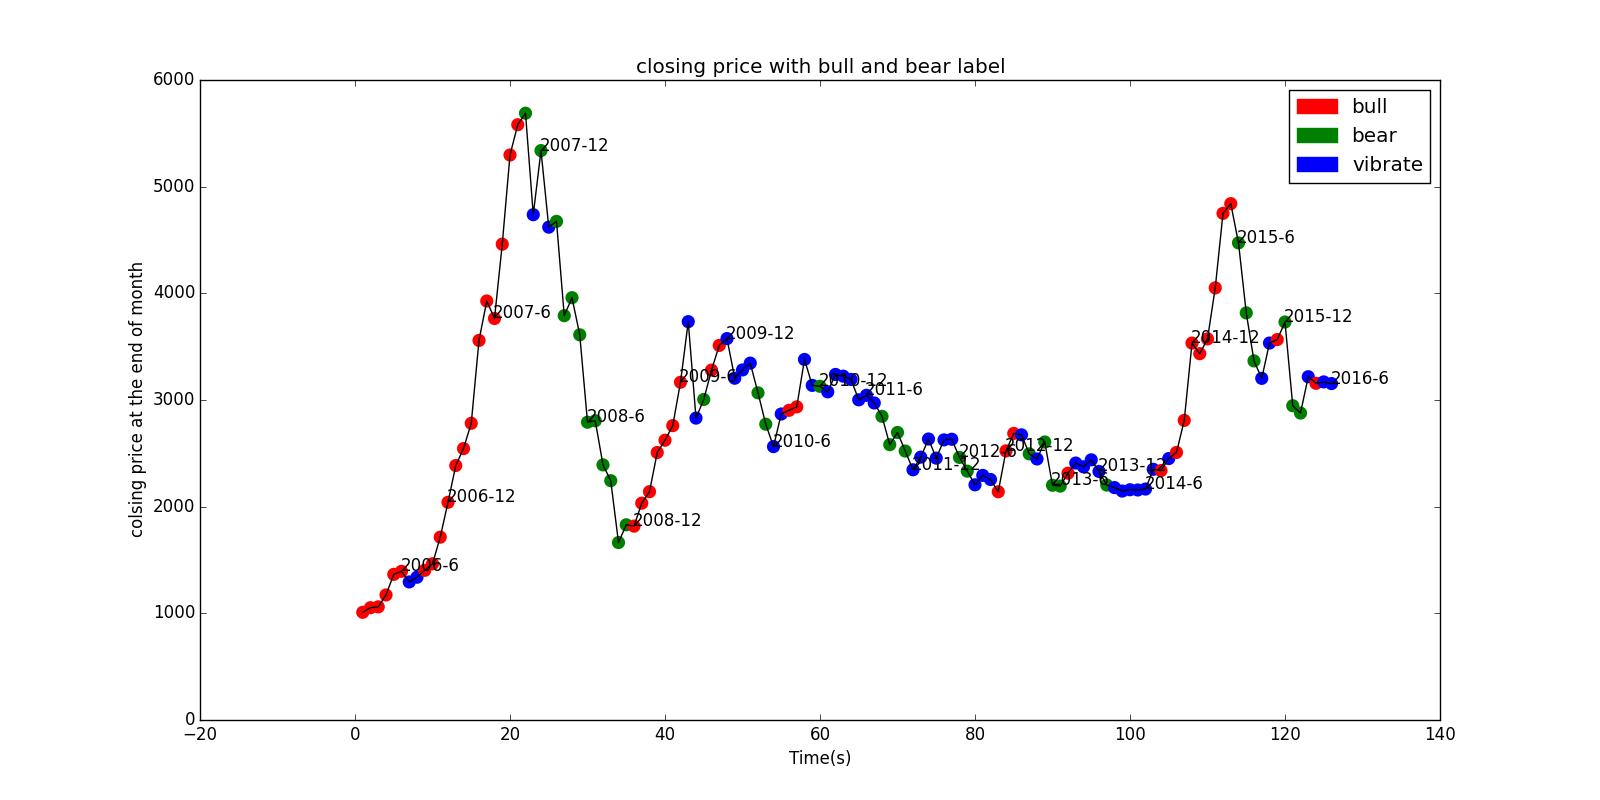
\includegraphics[width=1\textwidth]{标注可视化.png}
	\end{center}

\section{Result }
接下来我把试验结果可视化了,针对试验数据不足的情况(只有126个试验数据),我采用了留一交叉验证。具体的讲,就是每次用125个点训练模型,预测预留的点,循环126次。伪代码以及实验结果如下:
	\begin{lstlisting}[title=伪代码, frame=shadowbox]
	for i in ranges(0,126):
		for j in ranges(0,126):
			train data list.
			if j==i:
				get test data
			else:
				add data to train data list.
		end
		train model using train data
		predict test data using trained model
	end
	\end{lstlisting}
\begin{center}
	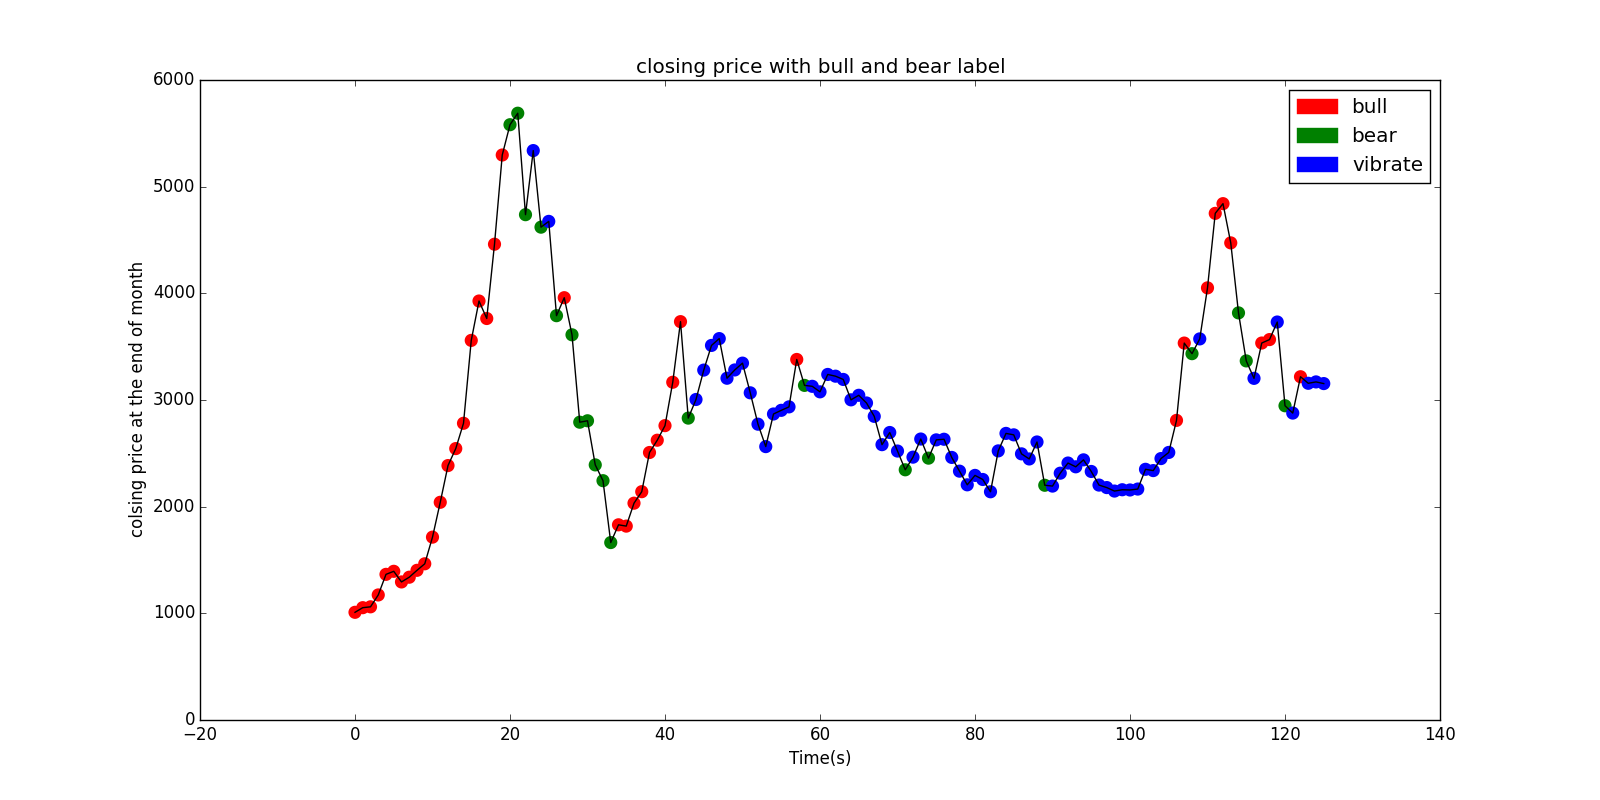
\includegraphics[width=1\textwidth]{测试结果可视化.png}
	\caption{利用留一验证方法得到的每个月的预测结果}
\end{center}
\begin{center}
	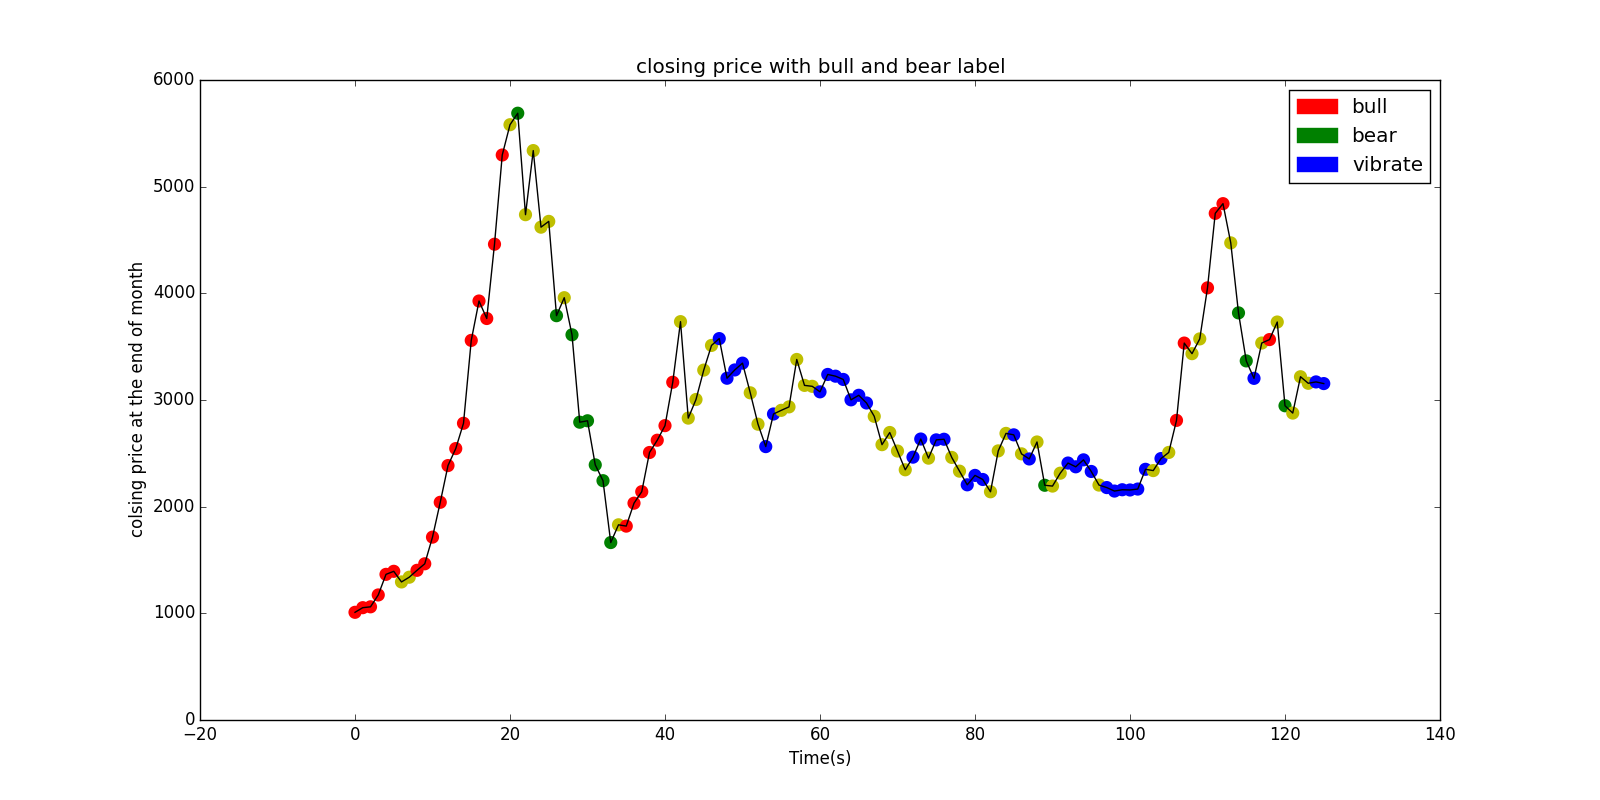
\includegraphics[width=1\textwidth]{测试结果可视化-带误分类标记.png}
	\caption{与数据标签不同的预测结果用黄色标注出来了}
\end{center}

从图中可以看出,模型在大牛市大熊市中表现很好,在10年到14年震荡的情况中表现较差。模型可以抓住大的机会,规避大的风险,但是对于小机会,小风险,把握能力不强。感觉目前的市场行情比较符合10年的情况,模型可能会一直判断为震荡市,针对这种情况,比较好的方法是利用10年到14年的数据重新训练一个模型,利用老模型提示大机会大风险,利用新模型重新分析老模型判断为震荡的情况,提高模型整体的效果。

\section{Improvement }
提高模型的效果,一个比较简单的方法是在数据上做文章,包括增大数据量以及提高数据的纯度。现在我们尝试提高数据的纯度。之前机器利用3\%方法自动标注的数据不一定准确,我们根据主观判断,手动更改数据的标签,使标注结果更加符合客观要求。标注结果如下图所示,我们希望得到的模型的分类效果能与这些标签尽量相同。\\
调整标签之后,预测的准确率有所提升,达到78.6\%。虽然指标看起来不是特别很高,但是考虑到标签本身存在的误差,以及月度的粒度比较大,实际的预测效果还是很不错的。调整后标签的分布更加合理,标签分布与数据的规律更加一致,可以预测的更准确。
\begin{center}
	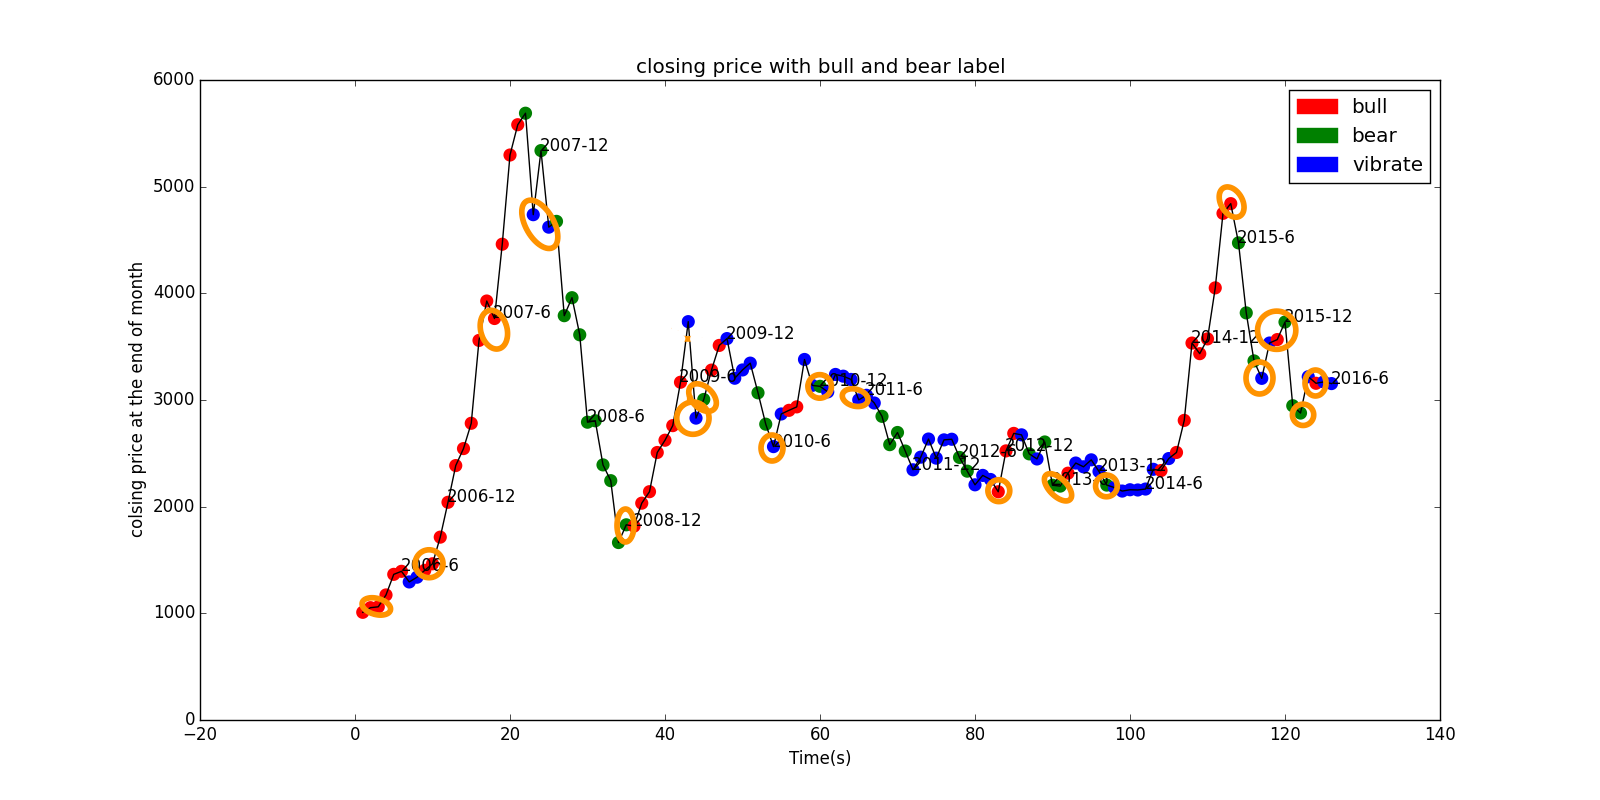
\includegraphics[width=1\textwidth]{需要调整的标签.png}
	\caption{橙色为需要手动调整标签的数据}
\end{center}
\begin{center}
	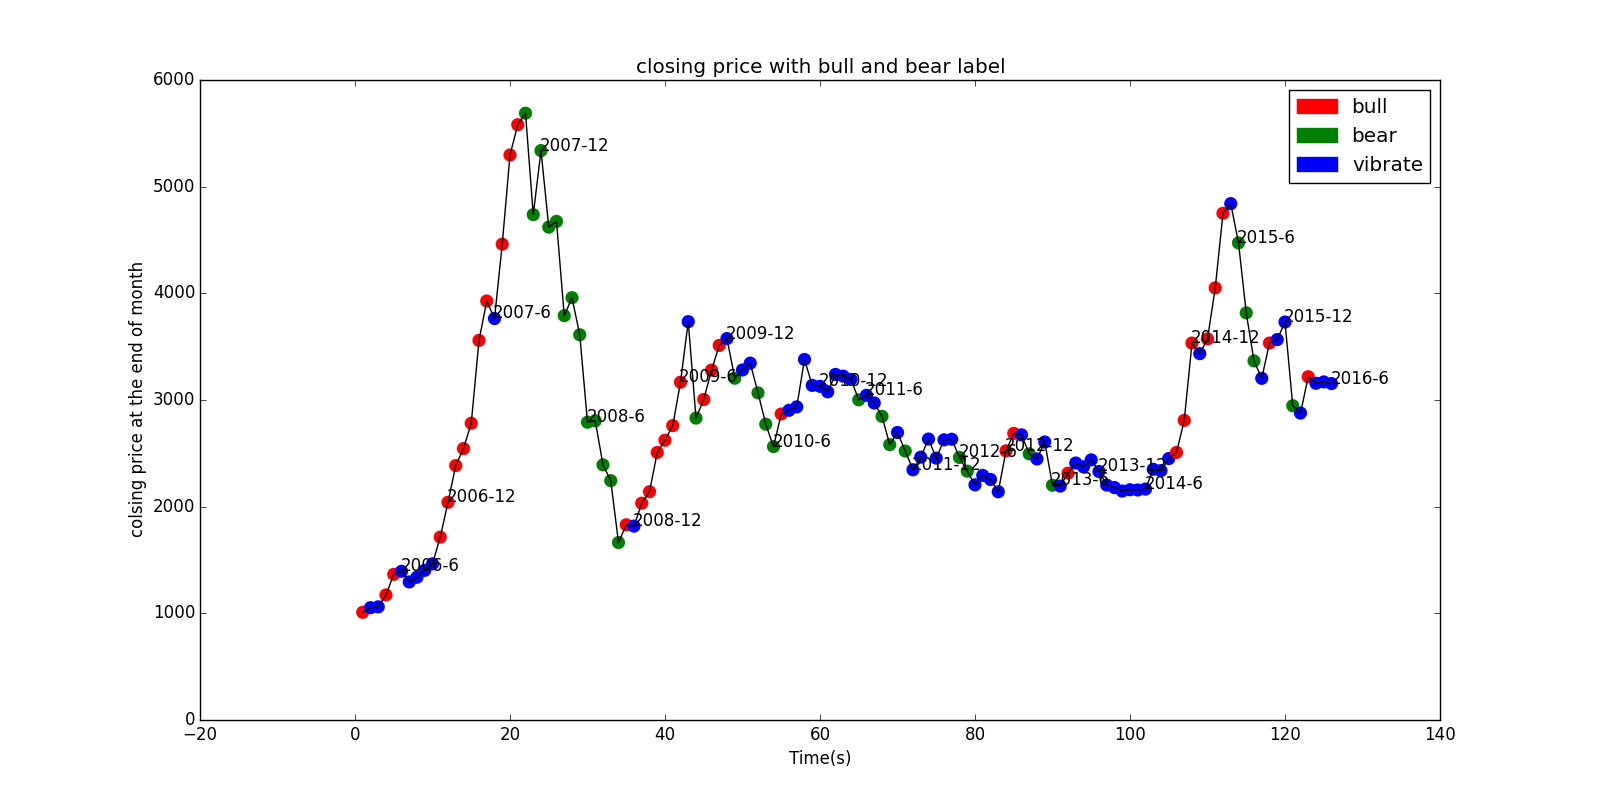
\includegraphics[width=1\textwidth]{调整后的标签.png}
	\caption{调整标签后的数据分布}
\end{center}
\begin{center}
	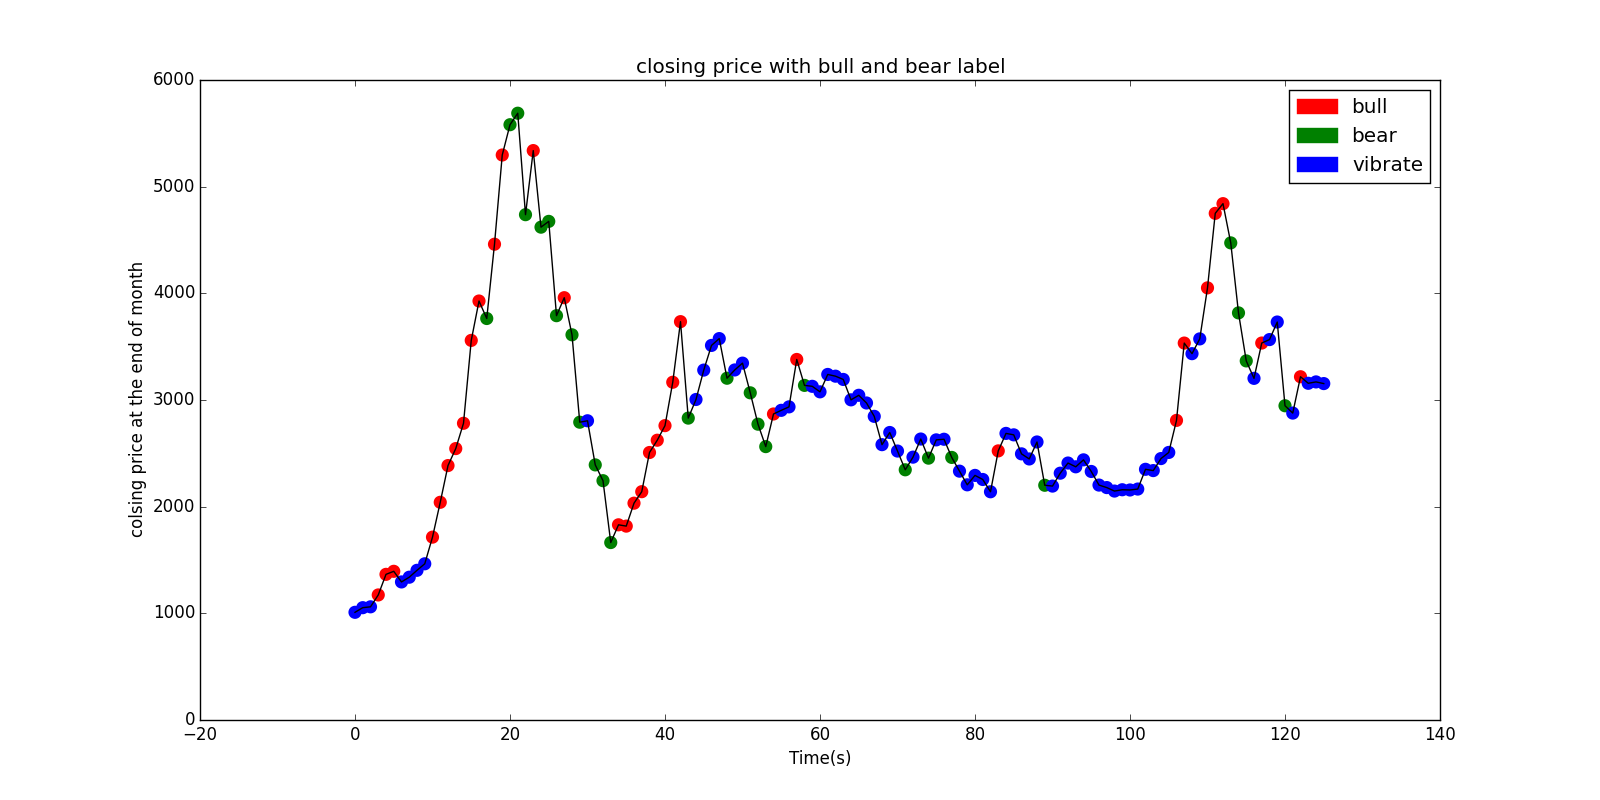
\includegraphics[width=1\textwidth]{第五次调整.png}
	\caption{调整标签后的数据分布}
\end{center}\begin{center}
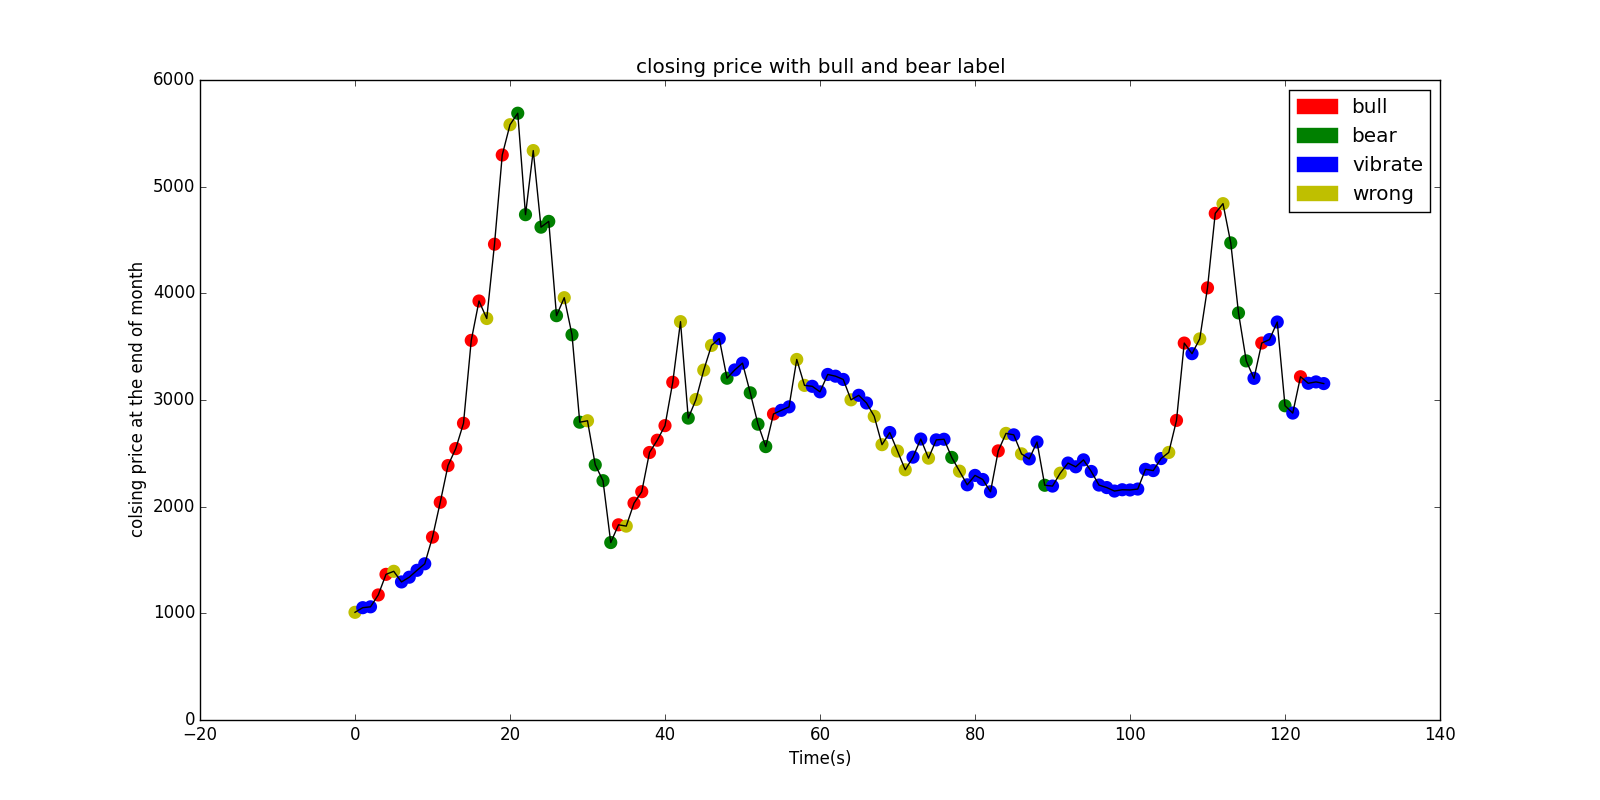
\includegraphics[width=1\textwidth]{第五次调整误差.png}
\caption{黄色标注出了跟标签不同的数据点}
\end{center}

\section{Data Automation }
数据自动化是一项比较麻烦的工作,可能遇到意想不到的bug,估计有两天到两周不等的工作量。所以在开始这项工作之前,可以先看一下可以通过API自动获取的数据在模型上的效果怎么样。利用留一交叉验证与重新标注的数据,我们得到了如下图的实验结果,最终的准确率是77.0\%.自动获取数据有三个很明显的优势:
\begin{enumerate}
	\item 可以自动获取过去时间每一天的数据,不在局限于月末的数据,大大扩充了数据集。
	\item 可以提取关于某一天当天、过去一周、过去一个月等不同时间粒度的信息,充分考虑了不同时间纬度的特征。
	\item 可以对模型的性能在过去的数据上做完备的测试。
\end{enumerate}
虽然较少的自动特征会损失稍许的精度,但是也带来了上述优势,如果能给自动获得的大量的数据添加有效的标签,相信可以进一步提升模型的性能,抵消掉特征量较少带来的损失。
\begin{center}
	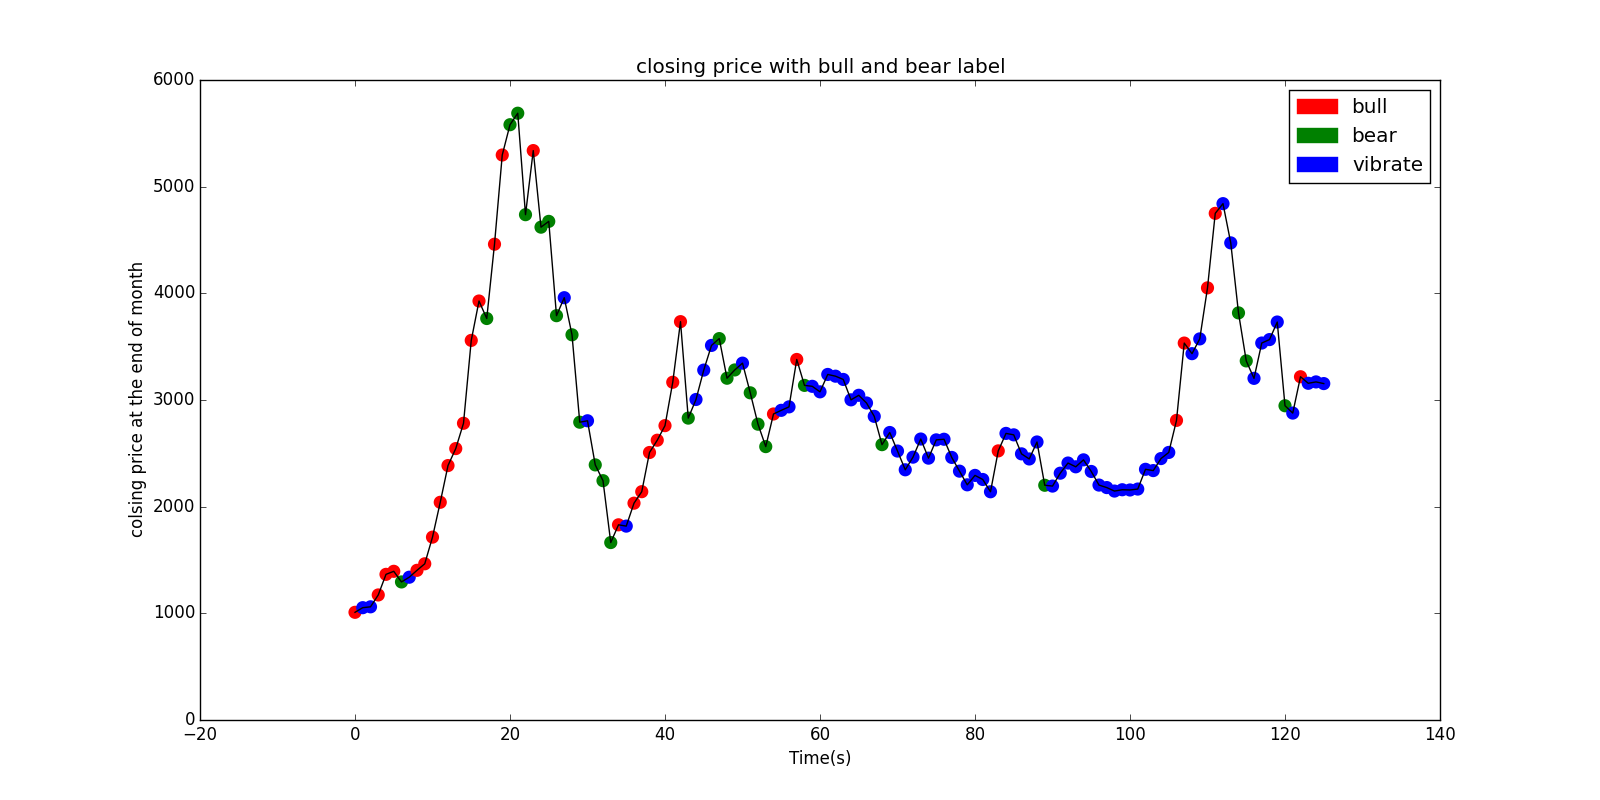
\includegraphics[width=1\textwidth]{四个特征第五次调整.png}
	\caption{四个特征驱动的模型的分类结果。}
\end{center}

%	\section{Criterion }
%	
%		\begin{equation}
%			\label{eq:u0}
%			\begin{aligned}
%				Score=E+ \alpha  \sum_{i=0}^{2}k_{i}p_{i}(x)logk_{i}p_{i}(x)
%			\end{aligned}
%		\end{equation}
	
\end{document}